% Things to be done before giving away for print
% - spell check
% - let others proof-read

\documentclass[a4paper,twoside]{report}

%% packages
%%%%%%%%%%%
\usepackage[utf8x]{inputenc}
\usepackage[USenglish]{babel}
\usepackage{amsbsy,amscd,amsfonts,amssymb,amstext,amsmath,amsthm,latexsym}
% Package mathpartir is currently not available in nixpkgs
\usepackage{mathpartir}
\usepackage{stmaryrd}
\usepackage{dot2texi}
\usepackage{tikz}
\usetikzlibrary{shapes,arrows}
\usepackage{url}
\usepackage[xindy]{glossaries}
\usepackage[nottoc]{tocbibind}
\usepackage{pdfpages}

\usepackage{todonotes}

%% options
%%%%%%%%%%
% Currently no such things seem to be needed.
% \newtheorem{definition}{Definition}
% \newtheorem{example}{Example}
% \newtheorem{lemma}{Lemma}
% \newtheorem{theorem}{Theorem}
% \newtheorem{claim}{Claim}
% \numberwithin{definition}{chapter}
\bibliographystyle{alphaurl}
\makeglossaries

%%% Local Variables:
%%% TeX-master: "../thesis"
%%% End:

%% macros
%%%%%%%%%
\newcommand{\loremipsum}{\todo[inline]{Lorem Ipsum}}

%% misc
%%%%%%%%%
\DeclareMathOperator{\pto}{\rightharpoonup}     % partial function arrow
\DeclareMathOperator{\powerset}{\mathcal{P}}    % powerset
\DeclareMathOperator{\proj}{\upharpoonright}    % projection
\DeclareMathOperator{\fst}{\pi_1}               % A x B → A
\DeclareMathOperator{\snd}{\pi_2}               % A x B → B

\def\naive{na\"{\i}ve}
\def\Naive{Na\"{\i}ve}
% Acronyms
%%%%%%%%%%
\newacronym{sdf}{SDF}{Syntax Definition Formalism}
\newacronym{ast}{AST}{Abstract Syntax Tree}
\newacronym{tptp}{TPTP}{Thousands of Problems for Theorem Provers}


%%% Local Variables:
%%% mode: latex
%%% TeX-master: "../thesis"
%%% End:


\begin{document}

% Title page
%%%%%%%%%%%%
\includepdf{titlepage.pdf}

\newpage
\thispagestyle{empty}
\mbox{}

% Erklärung
%%%%%%%%%%%
\input{include/erklaerung}

% Abstract
%%%%%%%%%%
\begin{abstract}
\documentclass{acm_proc_article-sp}

\usepackage[utf8]{inputenc}

\usepackage{cite}

\begin{document}

\title{A Language for the Specification and Efficient Implementation
  of Type Systems}

\numberofauthors{1}

\author{
\alignauthor
Pascal Wittmann
}

\maketitle

\begin{abstract}
  Type systems are important tools to ensure partial correctness of
  programs, to establish abstractions and to guide the programmer in
  the development process. However, there is currently a lack of
  established tools supporting the development of type systems, as
  there are for lexers and parsers. We introduce a declarative
  specification language for type systems, that allows to specify type
  systems in a natural deduction style. We generate from those
  specification two products. A first-order formula representation to
  facilitate the use of automated theorem provers and an efficient
  type checker. Both results aim to make the development cycle for
  type systems faster.
 \end{abstract}

\section{Motivation}
Type systems ensure partial correctness of programs or in other words,
they try to ensure that programs have meaning in the sense of the
semantics of the programming language. The type systems we investigate
are static type systems and can also be thought of as a static
approximation of the program semantics. Besides ensuring partial
correctness, type systems are means to establish abstractions, to
enforce adherence to these abstractions and they can serve as
documentation. All in all type systems can help to develop software
more efficiently (cf. \cite{Petersen:2014:ECS:2597008.2597152} and
\cite{Mayer:2012:ESI:2384616.2384666}).

Type systems are useful tools, if they fit to the programming language
and the application scenario. To ensure that they fit to the
programming language and the application scenario it makes sense to
adapt and modify existing type system or create new specialized type
systems. Those specializations can lead to better error messages, more
expressive type systems and the detection of more
errors, see \cite{Thiemann02programmabletype}. Currently there are, to our
best knowledge, no established tools that generate usable type
checkers from declarative specification languages. Those generators
could make the development of type checkers faster and less error
prone. Those generators would fit well into the language development
workbench besides the long established lexer and parser generators.

The other advantage of generating a type checker from a declarative
specification language is that the specification is close to the
formal description of the type system and the generation of the type
checker can be verified in the absence of a concrete
specification. Often not only the verification of the implementation
is a concern, but also that the type system satisfies certain
properties. As the proofs of propositions about type systems change
when the type system changes, it is desirable to make most of these
changes automatically. Therefore an other motivation for a type
checker generator is to translate specifications into first-order
formulas which can be fed into automated theorem provers to prove
propositions. This establishes a direct connection between the
specified type system, the proofs  and the generated type checker.

\section{Research Problem}
The research problem we are tackling is to create a tool that allows
to create an efficient type checker from a declarative specification
and that reduces the gap between formal reasoning about type systems
and their implementations. This problem splits up in smaller problems.

The first problem is the design of a declarative specification
language that is close to the formalisms used for type systems. This
language should make it easy to use existing syntax definition of
realistic programming languages and the difference between typing
rules on paper and in the specification language should be small.

The next problem is to investigate a good first-order formula
representation of specifications. This representation should be
designed such that it suits automated theorem proving and thus support
a fast prove search. It should also be investigated to which extend
theorem provers for first order logic can be used for type checking.

The main problem is the generation of an efficient type checker. The
performance of the resulting type checker should be comparable with
handcrafted type checkers and the generator should also be able to
cope with non-syntax directed typing rules in an efficient manner. In
this context it should be investigated whether facts proven by an
automated theorem prover can be exploited for the type checker
generation.
\section{Related Work}
There are early approaches for the generation of type checkers that
were not particularly designed for that purpose. For example the
Synthesizer Generator \cite{Reps:1984:SG:800020.808247} which uses
attributes grammars and the ASF+SDF Meta-Environment
\cite{vandenBrand:2001:AMC:647477.727788} based on conditional term
rewriting. Later approaches use similar techniques, for example TCG
\cite{phd/de/Gast2005} which uses inference rules, but are specialized
for the generation of type system. Those approaches have a lower
performance handcrafted implementations, because they implement the
control-flow implied by the used formalism.

A recent approach (TyC \cite{ortin2014automatic}) has focused on the
generation of type checkers for object-oriented programming
languages. It provides a framework to build efficient type checkers
for object-oriented languages (without polymorphism) and uses for this
purpose, in most parts, normal program code that implements an
interface to specify the type system.

Ott \cite{journals/jfp/SewellNOPRSS10} is an other approach that
generates from a specification language code for proof assistants and
\LaTeX, it tries to reduce the gap between the hand-written on-paper
proofs and machine checkable proofs.
\section{Approach}
Our approach tries to combine ideas from the related work presented
above. We design a high level declarative specification language that
is close to formalizations of type systems and generate first-order
formulas and efficient type checkers from it.

We use the language workbench Spoofax \cite{KatsVisser2010} for the
implementation of the specification language and the generators. We
use specifically two parts of Spoofax, the Syntax Definition Formalism
(SDF) to define new syntax and the transformation language Stratego to
generate code from specifications. 

When writing a specification, the syntax of the programming language
must be present in SDF. Specifications are organized in modules and
contain declarations of meta-variables, contexts, judgments and
rules. Figure \ref{fig:example-specification} gives and impression of a
specification.

\begin{figure}
\begin{verbatim}
module example
imports common
language simply-typed-lambda-calculus
meta-variables 	Term "~" { Type Exp }
                Ctx "$" { Context }
                Id "%" { ID }
contexts Context := ID{I} x Type{O}
judgments Context{I} "|-" Exp{I} ":" Type{O}.
rules

%x : ~T in $C
============== T-Var
$C |- %x : ~T

(%x : ~T ; $C) |- ~t : ~T
================================= T-Abs
$C |- \ %x : ~T . ~t : ~T -> ~T

$C |- ~t1 : ~T11 -> ~T12
$C |- ~t2 : ~T2
========================= T-App
$C |- ~t1 ~t2 : ~S
\end{verbatim}
\caption{Specification of the type system for the simply typed lambda
  calculus.}
\label{fig:example-specification}
\end{figure}

A stratego strategy transforms a specification into first-order
formulas in the TPTP\cite{Sutcliffe04tstpdata-exchange} format. The
use of the TPTP format allows to use a variaty of different automated
theorem provers. Typing rules are transformed into roughly into the
following format, where $p_1 \dots p_n$ are the premisses, $c$ is the
conclusion and $free$ collects free variables:

\begin{align}
  \forall v \in free(p_1, \dots, p_n, c) . p_1 \land \dots \land p_n \implies  c 
\end{align}

In this transformation process measurements are taken to ensure that
variables are correctly quantified and valid TPTP code is generated.

Stratego strategies generate the type checker as well. The generated
type checker consists of a constraint generator and a constraint
solver. We have chosen constraint solving as a basis for the type
checker, because it allows the generation of fast type checkers and is
not bound to certain class of type systems. To obtain a fast
constraint generator the structure of the rules should be analyzed,
also with the help of the formula generation and automated theorem
provers. A possible approach for dealing with non-syntax-directed
rules is for instance to check whether two rules commute.
\section{Contributions}
This work has three main contributions. It contributes a declarative
specification language that allows to specify arbitrary type systems
close to mathematical notation. A tool that transforms specifications
into first-order formulas in the TPTP format. Finally a tool that
generates an efficient type checker that can cope with
non-syntax-directed rules and uses automated proves to optimize the
resulting type checker. This reduces the amount of work to implement
type systems and reduces the gap between theory and practice. The
approach is also applicable to type systems from other areas, like
security.

The specification language and the formula generation are nearly
finished and tested with type systems for languages like PCF and
SystemF and with a type system for information flow security. The
generation of the type checker is, by the time of writing, work in
progress.
\bibliography{bibliography}{} \bibliographystyle{plain}
\end{document}

\end{abstract}

% Table of contents
%%%%%%%%%%%%%%%%%%%
\tableofcontents

\todo[inline]{Where do I put the "I would like to thank …"}
\todo[inline]{Search for a better word for 'goal'}
\todo[inline]{How do we refer to all the different types of
  languages? This should be done uniformly.}
\todo[inline]{Use glossary for abbreviations.}
\todo[inline]{``Mathematical'' or ``Formal''?}

% Content
%%%%%%%%%

\chapter{Introduction}
This chapter motivates the thesis, summarizes the contributions and
gives and overview of the structure of the thesis.

\section{Motiviation}
Type systems ensure that programs are well-behaved. In other words,
they ensure that programs have meaning in the sense of the semantics
of the programming language. The type systems we focus on are static
type systems and can be thought of as a static approximation of the
program semantics. Besides ensuring that programs are well-behaved,
type systems are means to establish abstractions and to enforce
adherence to these abstractions. Type systems can provide explicit
type annotations that serve as program documentation, which cannot
become obsolete. During type checking the program under consideration
can also be annotated with optimization hints for the compiler. All in
all type systems can help to develop software more efficiently
(cf.~\cite{Petersen:2014:ECS:2597008.2597152}
and~\cite{Mayer:2012:ESI:2384616.2384666}).

Type systems are useful tools, particularly if they fit to the
programming language and the application scenario. To ensure a type
system fits to a programming language, e.g.\ in the context of a
\gls{dsl}, it makes sense to adapt and modify existing type systems or
to create new specialized type systems. Those specializations can lead
to better error messages, more expressive type systems and the
detection of more errors
(cf.~\cite{Thiemann02programmabletype}). Currently there are only some
tools that support the creation and adaption of type systems by
generating type checkers from a type system specification
(\cite{Markstrum:2010:JDP:1667048.1667049}, \cite{ortin2014automatic},
\cite{gast2005generator}, \cite{tomb2005automatic} and
\cite{bergan2007typmix}), but they are not established. Such
generators accelerate the development of type checkers, make
development less error prone and fit well into the language
development workbench besides the long established lexer and parser
generators.

Type checker generators that use a high-level specification language
can also provide type theorists with a tool that allows them
experiment with new type systems without long development
delays. High-level specifications that are close to the formalism used
by type theorists have also the advantage of narrowing the gap between
type systems on paper and their implementation. Results shown for the
paper version can be adapted for the implementation (depending on the
correctness of the type checker generator). Such adaptions are not
possible with handcrafted implementations. High-level specification
languages are also suited to specify type systems from other areas,
like language-based information-flow
security~\cite{Sabelfeld:2006:LIS:2312191.2314769}.

To have more confidence into the properties of a type system, a
declarative specification can be translated into a first-order formula
representation, which can be used to conduct proofs of these
properties. As the proofs of propositions about type systems have to
change when the type system changes, it is desirable to make most of
these changes automatically. Automated theorem provers can try to
conduct those proves automatically. If the proof search fails one can
give hints for proof search, e.g.\ by providing induction
hypothesis. This establishes a direct connection between the specified
type system, the proofs and the generated type checker.

The goal of this thesis is to narrow the gap between theory and
implementation of type systems. A declarative specification language
is developed, in which type systems are represented close to the
standard formalisms. Two things are generated from those
specifications. First, a representation of the type system as
first-order formulas, intended to support proving properties of the
type system. Second, an efficient type checker that exploits facts
proven by automated theorem provers for optimization.

\section{Contributions}
The main contributions of this thesis are:
\begin{enumerate}
\item A declarative specification language for static type systems,
  with support for natural deductive style typing rules and error
  messages. The specification language is implemented in \gls{sdf} and
  capable of using most \gls{sdf} definitions of programming
  languages.
\item A transformation of type system specifications into equivalent
  first-order formula representations in the \gls{tptp} format. The
  first-order formula representations are suitable for typing
  checking, theorem proving and as a reference implementation for the
  type checker generator.
\item A generator that creates type checkers from type system
  specifications. This generator uses an intermediate representation
  for typing rules suitable for constraint generation and optimizes
  the intermediate representation using automated proofs, which check
  the applicability of an optimization.
\end{enumerate}

\section{Structure}
\todo[inline]{Describe how the thesis is structured.}

%%% Local Variables:
%%% mode: latex
%%% TeX-master: "../report"
%%% End:

\chapter{Preliminaries}
\section{Tools}
This section introduces the tools used in this thesis. We argue what
makes the tools suitable for achieving the goals of the thesis and
give a short overview of the alternatives.

\subsection{SDF}
\gls{sdf}~\cite{Heering:1989:SDF:71605.71607} is a formalism to define
the syntax of formal languages in the tradition of
\gls{bnf}. \gls{sdf} allows to define lexical and context-free
grammars and is, in contrast to \gls{bnf}, modular. This modularity
allows to compose \gls{sdf} syntax definitions. There are also parser
generators for \gls{sdf}, see~\cite{Rekers92parsergeneration}. In
contrast to formalisms for traditional parser generators like
Yacc\cite{Johnson75yacc:yet}, \gls{sdf} specifications are purely
declarative, which increases the reusability of the specifications.

The modularity of \gls{sdf} is a consequence of the fact that
\gls{sdf} is \textit{generalized LR
  parsable}\cite{Rekers92parsergeneration}. Generalized parsing means
that parsing might be indeterminate, i.e.\ the parser produces all
possibilities for syntactic ambiguities. This might not seem to be an
advantage, but generalized parsing has some nice implications. First,
the class of supported grammars is bigger and therefore enforces less
restrictions on the programmer and might allow a natural definition of
languages. Second, it enables the modularity of \gls{sdf}, because
composition of normal LR grammars is not guaranteed to be an LR
grammar again, but this is guaranteed for generalized LR grammars.

An other advantage is that \gls{sdf} is also scannerless
parsable~\cite{Brand02disambiguationfilters}, that means that
tokenization and parsing can be done in a single step.

\gls{sdf} also has support to specify layout sensitive
languages\cite{conf/sle/ErdwegRKO12} like Python or Haskell. Context
insensitive layout constraints are enforced at parse time and context
sensitive constraints are enforced at disambiguation time, i.e.\ all
ambiguities that violate layout constraints are removed.

\begin{figure}
\begin{example}{~}
\begin{lstlisting}[language=sdf]
module Bool
exports
  context-free start-symbols Bool
  sorts Bool
  context-free syntax
    "true"  -> Bool
    "false" -> Bool
    "~" Bool -> Bool {cons("Not")}
    Bool "&" Bool -> Bool {cons("And"),
                           layout("2.first.col < 2.left.col")}
\end{lstlisting}
\label{ex:sdf-grammar}
\end{example}
\end{figure}

Example~\ref{ex:sdf-grammar} shows a grammar that allows to write
conjunctions of \verb|true| and \verb|false|. Conjunctions are
represented in the \gls{ast} with the constructor \verb|And| and the
layout constraint enforces, that if conjunctions span over multiple
lines, the right-hand side of \verb|&| needs to be indented.

\gls{sdf} is used in this thesis to define the syntax of the
specification language for type systems and for the target
languages. Features like layout constraints make \gls{sdf} a good tool
for defining complex syntax for natural deduction rules. The
modularity and composability make it possible to define the syntax of
the specification language independent of the target language.
\subsection{Stratego/XT}
Stratego~\cite{Visser01} is a framework for the development of
transformation systems. It consists of the transformation language
Stratego and a set of tools (XT) for tasks like parsing and pretty
printing. The paradigm of Stratego is to use user-definable strategies
for rewriting. In Stratego distinguishes the following abstraction
levels.

\begin{description}
\item[Transformation rules] are basic rewrite rules on the structure
  of the \gls{ast}.
\item[Transformation strategies] are the glue between the
  transformation rules. They combine rules, define the order of
  application and the traversal order of the \gls{ast}. These
  strategies can be defined generically. \textit{scoped dynamic
    rewrite rules}~\cite{Visser01scopeddynamic} pass context
  information during the traversal, because normal rewrite rules are
  context-free.
\item[Transformation tools] allow to compile transformation strategies
  into a stand-alone program. The interface between such programs is
  the ATerm format for \glspl{ast}.
\item[Transformation systems] describe a set of programs created by
  the transformation tools, that form a source-to-source
  transformation usually including a parser and pretty printer.
\end{description}

Example~\ref{ex:stratego-module} shows a Stratego module that declares
the constructors from Example~\ref{ex:sdf-grammar}. It has one rule
\verb|Eval| that reduces a term one step. The strategy \verb|eval|
applies rule \verb|Eval| repeatedly from bottom to top.

\begin{figure}
\begin{example}{~}
\begin{lstlisting}[language=stratego]
module Bool
signature
  sorts Bool
  constructors
    Not   : Bool -> Bool 
    And   : Bool * Bool -> Bool
rules
  Eval : Not(True)      -> False
  Eval : Not(False)     -> True
  Eval : And(True, x)   -> x
  Eval : And(x, True)   -> x
  Eval : And(False, x)  -> False
  Eval : And(x, False)  -> False
strategies
  eval = bottomup(repeat(Eval))
\end{lstlisting}
\label{ex:stratego-module}
\end{example}
\end{figure}

Stratego interacts well with \gls{sdf} and has facilities to integrate
nicely into tool-chains. In addition it allows to write abstract and
generic transformation. That makes it a good choice for the
transformation system.
\subsection{Spoofax}
Spoofax\cite{KatsV10} started with the goal to provide an \gls{ide}
for \gls{sdf} and Stratego. It was then developed to a language
workbench for Eclipse that allows language development with editor
support for both, the languages used for development and the developed
language. Spoofax allows smooth switching between both editor
services. The editor for the developed language can be deployed
standalone. Those editor services can provide syntactic and semantic
analysis based on live parses, with error recovery and origin
tracking. Those facilities are implemented language pragmatic, which
allows developers to focus on language specific parts.

We use Spoofax in this thesis to provide editor support for the
specification language and as glue between \gls{sdf} and Stratego in
the development of the specification language, the formula generator
and the type checker generator.
\subsection{Vampire}
We use the automatic theorem prover Vampire~\cite{VoronkovVampire} to
proof classical first-order logic propositions about type system
specifications. Vampire is able to parse formulas in the \gls{tptp}
format and provides detailed output for the conducted proofs. We use
this output to extract information about the applied axioms, which are
in our case typing rules.
\subsection{Alternatives}
\section{Type Systems}
\textit{Type theory} started as an attempt by Gottlob Frege to solve Russel's
paradox, that shows that \naive{} set theory is inconsistent. Frege
argued that a predicate requires an object as argument and cannot have
itself as an argument, as it is the subject.\todo{Make this more
  precise} So the initial motivation for type theory was to avoid
paradoxes and contradictions in logics and rewrite systems. The term
\textit{type system} refers to type theories whose logics rewrite
systems are programming languages. Type systems address therefore
similar problems as general type theory. The problem they address is
to ensure that programs have meaning, whereas in type theory the
problem is the ensure the consistency of a logic.

What does it mean to ``ensure that programs have meaning''. First, it
means that one wants to filter the useful programs. It is not useful
to have a syntactically valid program that has no semantics. This is
done by assigning types to the expressions of the program. A
\textit{type checker} can then check, whether those types match with
the expressions. If the type checker succeeds the program is
\textit{well-typed} and has meaning. Second, a type system allows to
establish abstractions through user definable data types. When type
checking a program, it is also ensured that those abstractions are not
violated.\footnote{This is only true for so called ``strong'' type
  systems.} In this thesis \textit{static} type systems are
considered. In a static type system types are checked prior to
execution. This early checks can provide guarantees about the programs
behavior 
\section{First-Order Logic}

%%% Local Variables: 
%%% mode: latex
%%% TeX-master: "../report"
%%% End: 

\chapter{Specification Language}
\label{cha:spec-lang}
Our type system specification language is a \gls{dsl} for people
familiar with type systems or type theory. While developing it, we had
the following goals in mind that will be described below. The
specification language should be

\begin{itemize}
\item close to text-book formalisms used in the type system community
\item purely declarative
\item modular
\item usable with existing syntax definitions of programming languages
\end{itemize}

Those characteristics fit well with the goals of making it easy to
experiment with type systems and to create type systems from a
high-level specification.
\section{Design \& Architecture}
\label{sec:design--architecture}
In this sections we introduce the architecture of the specification
language with references to a small examples and argue how this
architecture reflects the goals mentioned above.

Specifications in our specification language are divided into eight
sections, of which two are optional. The sections have to be present
in the order they are introduced.

\paragraph{Module name} The first section declares the name of the
specification module. This name is a unique identifier and used for
imports.

\paragraph{Imports} The second section declares which other type
system specifications are imported and is optional. It is possible to
prevent sections of a module from being imported. Sections that shall
be excluded have to be listed in parenthesis after the module name.

\begin{example}{}
\begin{lstlisting}[language=sltc]    
import some-specification (language contexts)
\end{lstlisting}
\label{ex:import-section}
\end{example}

Example~\ref{ex:import-section} imports the specification module
\code|some-specification| without the sections \code|language| and
\code|contexts|.

\paragraph{Language} The third section declares the language for which
a type system should be specified. This language needs to be present
as an \gls{sdf} module located at the specified path. We call this
language from now on \emph{target language}. If other modules are
imported the target language must be defined only once.

\begin{example}{~}
\begin{lstlisting}[language=sltc]
language specifications/simply-typed-lambda-calculus/syntax
\end{lstlisting}
\label{ex:language-section}
\end{example}

In Example~\ref{ex:language-section} the language definition at
\code|specifications/simply-typed-lambda-calculus/syntax.sdf|
is used, this path is relative to the \code|syntax| folder of the Spoofax
project.

\paragraph{Contexts} The fifth section declares the contexts that can
be used in the judgments and rules. Informally these contexts are
declared as cross-products of non-terminals, i.e.\ a context is a set
consisting of tuples of terminals that can be produced by the
non-terminals in the declaration. Every context has a name, which can
be used as a non-terminal in the specification.

Contexts serve in most use cases as bindings for variables. Therefore
it is necessary to be able to look up terminals in a context. In the
context declaration each non-terminal is annotated with an input
(\code|{I}|) and output \code|{O}| tag. Those tags specify the key and
value positions of the context. Depending on those annotations we
generate look up functions. If all non-terminals are tagged as inputs
the generated look up function will perform a normal membership
test. However a context with only output tags is not useful as it is
not possible to add elements to it.

Given a context declaration \code|Z := A{I} x B{I} x C{O} x D{O}| an
instance of this context looks like \code|(a : b : c : d) ; z| where
\code|a|, \code|b|, \code|c| and \code|d| are terminals produced from
the non-terminals \code|A|, \code|B|, \code|C|, \code|D|,
respectively. \code|z| is an other instance of context \code|Z| or the
empty context, which is written \code|()|.

\begin{example}
\begin{lstlisting}[language=sltc]
contexts Binding := ID{I} x Type{O}
\end{lstlisting}
\label{ex:context-section}
\end{example}

Example~\ref{ex:context-section} shows a context called \code|Binding|
that consists of a non-terminal \code|ID| tagged as input and a
non-terminal \code|Type| tagged as output. This contexts models a type
binding for identifiers. We generate from this context declaration a
look up function of the form \code|i : t in c| where \code|i|
represents a terminal produced from \code|ID|, \code|t| a terminal
produced from \code|Type| and \code|c| represents an instance of
context \code|Binding|. 

\paragraph{Meta-variables} The fourth section declares
meta-variables. In specifications meta-variables are used to refer to
expressions of the target language and to contexts. The declaration of
a meta-variable consists of a class, a prefix and a set of
non-terminals from the target language. We use the class to
distinguish different kinds of meta-variables. Currently we use
classes only for merging meta-variable declarations when resolving
imports. For details see~\ref{sec:generate-sdf}.

The set of non-terminals defines the scope of a meta-variable. Every
non-terminal from the target language contained in this set is
extended with meta-variables. In other words, a meta-variable is a
substitute for every terminal that can be produced from one of the
non-terminals. We explain the extension of the target language in
detail in Section~\ref{sec:generate-sdf}.

Syntactically a meta-variable is a string of numbers and letters that
is prefixed with the prefix of the meta-variable definition. The sole
purpose of the prefix is to avoid syntactic ambiguities. The prefix
itself can consist of numbers, letters and the following symbols
\code|~|, \code|$|, \code|%|, \code|&| and \code|?|. %% $
There is currently no way to add new symbols to that list, but editing
the syntax definition of the specification language. Usually a prefix
is chosen such that it is not a prefix of a construct of the target
language.

\begin{example}{~}
\begin{lstlisting}[language=sltc]
meta-variables 	Term "~" { Type Exp }
                Ctx "$" { Context }
                Id "%" { ID }
\end{lstlisting}
\label{ex:meta-variable-section}
\end{example}

Example~\ref{ex:meta-variable-section} declares three classes of
meta-variables. The first class is called \code|Term| and each
meta-variable of this class has the prefix \code|"~"|. Productions for
meta-variables of this class are added to the non-terminals
\code|Type| and \code|Exp|.

\paragraph{Judgments} The sixth section of a type system specification
module declares judgments. In our specification language judgments are
the basic building blocks of the rules defined in the next
section. This is common in the specification of deduction systems in
general. Judgments can be thought of as the ``syntax'' of the type
system, the semantics is defined by the rules.

A judgment can be defined rather arbitrarily from a combination of
strings of letters and numbers, non-terminals of the target language
and the names of the contexts. Those can be mixed freely, as long as a
string separates the non-terminals and context names. This restriction
is only needed to reduce the number of syntactic ambiguities in the
language. Judgments do not have a name as it is not possible to
quantify over them. To separate judgment declarations from each other,
each declaration must be finalized with a dot.

Non-terminals of the target language and context names need to be
annotated with input/output-tags. Those tags describe which parts of
the judgment need to be computed by rule applications and which are
provided as input parameters to the rule application. Contexts
currently only support the input tag.

\begin{example}{~}
\begin{lstlisting}[language=sltc]
judgments Context{I} "|-" Exp{I} ":" Type{O}.
          Type{I} "<:" Type{I}.
\end{lstlisting}
\label{ex:judgment-section}
\end{example}

Example~\ref{ex:judgment-section} shows two judgments. The first could
be the typing judgment of a variant of the simply typed lambda
calculus with a context and an expression of the target language as
input and a type of the target language as output. The second judgment
defines a relation between the types of the target language, i.e.\ it
has only input positions. This judgment could represent a subtyping
relation.

\paragraph{Rules} The seventh section of the module declares the
(typing) rules. These rules define the semantics for the judgments
declared in the previous section. The syntax of the rules replicates
the form of inference rules: A (possibly empty) list of premises
separated from a conclusion by a horizontal line. Premises and
conclusion are instantiated judgments. All meta-variables that occur
free in rules are implicitly all-quantified. This means that all
meta-variables are all-quantified, as there is no mechanism to bind
variables in typing rules.

Rules can be annotated with a name. The names increase the readability
of the specification and allow to create human readable derivation
traces. The rules have also support for custom error messages. There
are two kinds of error annotations. Premises can be annotated with
\code|@error msg|, where \code|msg| can contain meta-variables and
holes (written \code|{}|) interleaved with arbitrary strings. Those
errors are thrown if the premise could not be derived or if the
calculated output does not match the expected output. The
meta-variables are instantiated with the appropriate terms and the
hole with the expected output. The other kind of errors are prefixed
with \code|@implicit| and are thrown if an implicit equality between
two meta-variables cannot be satisfied. The meta-variables are
distinguished in the error message by \code|@[number]| annotations,
where \code|number| is a natural number. The conclusion can also be
annotated with error messages for implicit
equalities. Section~\ref{sec:constr-gener} and
Section~\ref{sec:constraint-solving} explain how error messages are
implemented in the type checker generator.

\begin{example}{~}
\begin{lstlisting}[language=sltc]
judgments
TermBinding{I} "|" TypeBinding{I} "|-" Exp{I} ":" Type{O}.
Type{O} "= [" ID{I} "->" Type{I} "]" Type{I}.

rules

===================== Subst-Eq
~S = [ %x -> ~S ] %x@1    @implicit %x " does not equal " %x@1.


~U = [ %x -> ~S ] ~T @error ~U "is not" ~T "where" %x "is
                            replaced by" ~S.
$C1 | $C2 |- ~e : all %x . ~T 
@error ~e "should have type all" %x "." %~T "but has type" { }.
============================== T-Tapp
$C1 | $C2 |- ~e [ ~S ] : ~U
\end{lstlisting}
\label{ex:rules}
\end{example}

Example~\ref{ex:rules} shows the rules \code|Subst-Eq| and
\code|T-Tapp| from the SystemF \todo{Reference}
implementation. \code|Subst-Eq| has no premises and an implicit
equality in the conclusion. Rule \code|T-Tapp| shows how the expected
output is used in the error messages and how premises are annotated
with error messages. All error message annotations belong to the
preceding premise.

\paragraph{Conjectures} Tests for a specification are called
\textit{conjectures}. Their syntax is similar to the syntax of rules,
with two exceptions. It is not possible to annotate premises or
conclusions with error messages and a conjecture can be marked as
\textit{not derivable} by prepending the separating line with a
slash. Marking conjectures not derivable allows to formulate negative
tests.

\begin{example}{~}
\begin{lstlisting}[language=sltc]
============================
() |- let fac : int -> int = 
  fix f : int -> int (
    fun n : int (
      ifz n then 1 
      else n * (f (n - 1))
    )
  )
 in (fac 3) : int

/===========================
() |- fun x : int (x) : int
\end{lstlisting}
\label{ex:conjecture-section}
\end{example}

Example~\ref{ex:conjecture-section} shows two conjectures of the PCF
implementation. They use the judgment shown in
Example~\ref{ex:judgment-section}. The first conjecture asserts that
the type of the faculty function applied to \code|3| is \code|int| and
the second conjecture asserts that \code|fun x : int (x)| has type
\code|int| is not derivable.

Line comments (\code|//|) and block comments (\code|/* ... */|) can be
inserted everywhere in the module.

How does this design reflect the characteristics from the beginning of
this chapter? We will address this point by point.

\begin{description}
\item[Usage] Formal definitions of type systems usually consist of
  judgment, rules and auxiliary definitions for contexts. All those
  elements can be represented in a natural way in the specification
  language. Judgments can be defined as an arbitrary combination of
  non-terminals and separation symbols, as long as the syntax does not
  create ambiguities. Rules are written in a natural deduction style,
  because this is the most common representation of typing rules and
  it acknowledges the deductive nature of typing rules in
  general. Contexts can be defined using a set like notation. This is
  close to the intuitive semantics of contexts and allows to generate
  commonly used syntax.
\item[Declarative] Everything that can be defined in the specification
  language has no side effects or possibilities to embed executable
  code.
\item[Modularity] Type system specifications are organized in
  composeable modules. A module can import other modules or even only
  parts of other modules. This enables the reuse of existing type
  specifications and the separation of orthogonal features.
\item[Integration] Type systems can be defined for every programming
  language for which a \gls{sdf} syntax definition exists. These
  definitions can be used in most cases without further
  modifications. One of the requirements is that they introduce a
  constructor for every context-free production. Modifications are
  also needed if one wants to use a language concept inductively in
  the type system, but has not implemented this concept with explicit
  induction in the syntax. The implementation of records in the simply
  typed lambda calculus is an example for this. \todo{Reference}
\end{description}
\section{Implementation}
\label{sec:generate-sdf}
In this section we describe how the specification language is
implemented and how the new syntactic constructs that can be defined
in a specification are integrated.

The specification language itself is defined in \gls{sdf} and consists
of four \gls{sdf} modules. The module \code|Common| which consists of
lexical definitions that are used in multiple modules, the module
\code|BaseLanguage| which defines the syntax of the specification
language, the module \code|Generated| which contains new syntax that
was defined in a specification and the main module \code|SLTC| that
combines the previous modules.

The module \code|Common| only defines character classes and lexical
restrictions therefore we will not explain it in detail.

The syntax of the specification language, which is independent of the
target language, is defined in the module \code|BaseLanguage|, which
is parameterized by the non-terminals \code|TypingJudgment| and
\code|MetaVariable|. These non-terminals depend on the actual target
language and are therefore defined in \code|Generated|.

In a new project the module \code|Generated| does not exist in the
syntax folder, as no specification is in use. Building a project
copies a dummy \code|Generated| module from the resource folder into
the syntax folder. Module \code|Generated| contains empty productions
for the non-terminals \code|TypingJudgment| and \code|MetaVariable|
and it ensures that a compilation of the whole project is possible
without a specification (e.g.\ to run tests). The strategy
\code|toSdf| generates a specification specific \code|Generated|
module.

The strategy \code|toSdf| transforms a specification into a \gls{sdf}
\gls{ast} which is then pretty printed and saved in the syntax
folder. The generated module \code|Generated| imports module
\code|Common| and the \gls{sdf} file of the target language. Module
\code|Generated| also contains context-free grammars for context,
meta-variables and judgment declarations.

For each context declaration the strategy \code|make-contexts|
generates productions for the empty context, context bindings and
context look ups. Figure~\ref{fig:context-productions} shows the
resulting productions. Furthermore \textit{Name} is the name of the
context declaration and \code|n| the position of the context
declaration.

\todo{Increase space between figures}

\begin{figure}
\begin{grammar}
  <Name> ::= `ContextEmpty-n'
  \alt `ContextBind-n' <Elem> <Name>
  \alt `ContextLookup-n' <Elem> <Name>
  \alt `(' <Name> `)'

  <Elem> ::= <String> | <String> `:' <Elem>
\end{grammar}
\caption{Context productions}
\label{fig:context-productions}
\end{figure}

Figure~\ref{fig:meta-variable-productions} shows the productions
created by \code|make-variable| for meta-variables. A meta-variable
consists of its prefix, a name and of an optional error
annotation. There are two productions for meta-variables. The first
extends the non-terminal \textit{Scope} of the target language and the
second enables the use of meta-variables in error messages. In the
constructor of meta-variables \code|m| is either the context number in
case \textit{Scope} is a context and otherwise the meta-variable
class.

\begin{figure}
\begin{grammar}
  <Scope> ::= `MetaVariable-m' <Prefix> <MetaVariableName> <Anno>

  <MetaVariable> ::= `MetaVariable-m' <Prefix> <MetaVariableName>
  <Anno>

  <Anno> ::= $\epsilon$ | `@' <ErrorNumber>
\end{grammar}
\caption{Meta-variable productions}
\label{fig:meta-variable-productions}
\end{figure}

Strategy \code|make-judgment| creates productions for judgment
declarations. For each judgment we generate a production that consists
of all non-terminals separated by the separators from the
declaration. In case of a built-in the constructor of the constructor
has the name of the built-in, otherwise it is the judgment position
append to the string \code|TypingJudgment|.

The module \code|SLTC| plugs all modules together. It imports the
module \code|Generated| and instantiates the parameters of module
\code|BaseLanguage|.

%%% Local Variables: 
%%% mode: latex
%%% TeX-master: "../report"
%%% End: 

\chapter{Formula Generation}
When developing type systems it is desirable to be able to prove
propositions about those type systems. Those help to understand the
type system better and help to prevent errors. Those propositions are
often proven by hand, but those proves are error prone, hard to extend
and time expensive. Prove assistants help to gain extensibility and
eliminate error. Using automated prove assistants can reduce the time
effort for suitable propositions. This chapter describes how
first-order formulas are generated from type system specifications and
that these formulas can be used to type check programs.
 
\section{Goals}
\section{Why First-Order Logic?}
\subsection{Expressiveness}
\subsection{Tool-Support}
\section{Translations}
For the generation of first-order formulas not all sections of a
specification are important. The section that declares the
meta-variables and the section that declares the judgments are not
used directly at all. With regard to formula generation they are only
used to ensure correct syntax.

\todo[inline]{Implement imports and describe how they are handled.}

Environments declarations are translated in a uniform way. For every
environment two formulas are generated. These two formulas handle the
look-up of entries in the environment. One formula for the base case
and one for the step case of the lookup.

\begin{multline}
  \forall e, x_1, \dots, x_n, y_1, \dots, y_m . \\ (lookup_e(x_1,\dots,x_n,y_1,\dots,y_m, bind(x_1,\dots,x_n,y_1,\dots,y_m,e)))
\end{multline}

The above formula represents the base case of environment
look-ups. All non-terminals in the environment definition tagged with
input are translated into variables $x_1 \dots x_n$ and all tagged
with output are translated into variables $y_1 \dots y_m$
respectively. The variable $e$ ranges over all possible
environments. The $bind$ predicate used in this formula allows to add
new input/output pairs to the environment. In the implementation the
order of arguments is a bit different, but this difference is for the
discussion of the concept negligible. For details see the next
section.\todo{Use a reference} The predicate $lookup$ that is defined
also takes input/output pairs and an environment. In the base case the
environment given to $lookup$ contains the input/output pairs of
$lookup$ directly. Therefore those are trivially contained in the
environment.

\todo[inline]{Format look-up step formula nicely.}
\begin{multline}
  \forall e, x_1, \dots, x_n, x_1', \dots, x_n', y_1, \dots, y_m, y_1', \dots,
  y_m' . \\
  (lookup(x_1, \dots, x_n, y_1, \dots, y_m, e) \implies \\ lookup(x_1,
  \dots, x_n, y_1, \dots, y_m, bind(x_1',\dots,x_n',y_1',\dots,y_m',e))
\end{multline}

This formula represents the step case of environment look-ups. Its
intuition is that if some input/output pair is contained in an
environment $e$ the it is also contained in an environment in which a,
possibly different, input/output pair is stored. Variables $x_i$ and
$x_i'$ are non-terminals from the environment declaration tagged with
input, $y_i$ and $y_i'$ are non-terminals tagged with output
respectively.

The AST nodes of the programming language are translated into
predicates. To help theorem provers for each of those predicates an
axiom for injectivity and univalence is created. Those hold by
definition of the AST nodes.

The most important part is the translation of the typing
rules. Depending on whether the typing rules has premises either of
the following schema is used:

\begin{align}
  &\forall FV(c) &.\,& c \\
  &\forall FV(p_1,\dots, p_n) &.\,& p_1 \land \dots \land p_n \implies c
\end{align}

\todo[inline]{In the following free variables are actually free
  meta-variables.}
The meta-variables $p_i$ are the premises and $c$ is the conclusion of
the typing rules. The intuition of a typing rule is that the
conclusion can be derived if all premises can be derived. In terms of
first-order logic ``derived'' means for arbitrary formulas that there
is a proof and for predicates that the predicate holds under the given
interpretation. Therefore a typing rule without premises is translated
into a formula that consists of the conclusion and all-quantifies all
free variables of the conclusion. Free variables are all-quantified,
because all possible variants of the conclusion have to be derivable.
Typing rules with premises are translated into a single
implication. The premise of the implication is the conjunction of all
premises of the typing rule. This ensures that all premises need to be
derivable/satisfied. The conclusion of the implication is the
conclusion of the typing rule. This makes sense as the intuition was,
that the conclusion of the typing rule is derivable if all premises
are derivable, which is exactly the semantics of this implication.

Type judgments are translated into simple predicates. Equality and
inequality can be expressed via judgments with the annotation ``is
Eq'' and ``is Neq'', respectively. Those judgments must have exactly
two non-terminals.
\section{Implementation}
The implementation details of the translation from the specification
language into first-order formula is described in this section.

\todo[inline]{Extend for imports.}
The implementation is organized in the following steps. Fist, the
module is split up into its components. Those are: module description,
programming language, meta-variables, environments, judgments, typing
rules and conjectures. 

\section{Performance}
%%% Local Variables: 
%%% mode: latex
%%% TeX-master: "../report"
%%% End: 

\chapter{Type Checker Generation}
\todo[inline]{Terminology: Type Checker vs. Type Inference}
\section{Goals}
This section briefly describes and motivates the design goals of the
type check generator.

The first goal is to produce fast type checkers, even if the type
system specification is not geared towards performance. Mainly this
means to try to deal with non-syntax directed typing rules without
backtracking. The motivation for this is, that non-syntax directed
typing rules are often more readable and changes have mainly local
effects.

The second goal is to design a modular type checker generator. A type
checker generator that can be easily adapted and that facilitates the
exchange of components. This modularity is desirable because it
increases the reusability and makes it possible to combine projects.

The third goal is to generate type checkers emit readable error
messages if a program is not well-typed. This is essential to make the
type checker usable in any way.
\section{Architecture}
\todo[inline]{Describe more explicitly that we use constraint solving}
The type checker generator has two phases: Template generation and
template optimization. In the template generation phase the type
system specification is transformed with minor modifications into
templates. A template is different representation for a typing rule,
which is better suited for type checking. Templates will be introduced
in detail in Section~\ref{sec:constraint-templates}. In the template
optimization phase, those templates are optimized. Those optimizations
aim to reduce the amount of non-determinism in the type system and
therefore reduce the amount of backtracking in the type checker. The
end product after those two phases, is a file that contains the
optimized templates.

The templates are the input for the next two phases, which are located
in the type checker. Instead of generating the type checker directly
from the specification, a generic type checker is that takes the
templates as input. The generic type checker has two phases:
Constraint generation and constraint solving. The constraint
generation phase has the templates and the program expression that shall be type
checked as inputs. To generate the constraints the program expression
is traversed according to the templates and the emitted constraints
are collected. Those constraints are then solved in the constraint
solving phase.

The four phases correspond to modules. Each phase has a well-defined
interface, therefore the implementation can be exchanged freely. This
makes it possible to use different constraint solvers, constraint
generators or template optimizers.

\begin{figure}
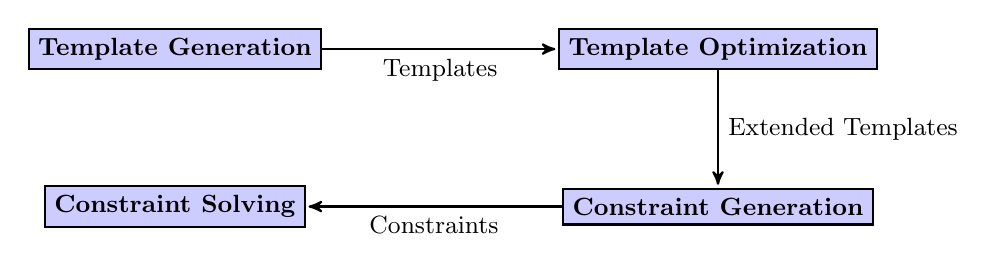
\begin{tikzpicture}[->,>=stealth',shorten >=1pt,auto,align=center,node distance=2cm,
  thick,main node/.style={rectangle,fill=blue!20,draw,font=\small\bfseries}]

  \node[main node] (1) {Template Generation};
  \node[main node] (2) [right=3cm of 1] {Template Optimization};
  \node[main node] (3) [below of=2] {Constraint Generation};
  \node[main node] (4) [below of=1] {Constraint Solving};

  \path[every node/.style={font=\small}]
    (1) edge node [right, below] {Templates} (2)
    (2) edge node [right] {Extended Templates} (3)
    (3) edge node [right, below] {Constraints} (4);
\end{tikzpicture}
\caption{Phases of the type checker generator}
\label{fig:phases}
\end{figure}
\section{Implementation}
\label{sec:implementation}
The following sections describe the implementation of the type checker
generator, one section per phase.

\subsection{Constraint Templates}
\label{sec:constraint-templates}
In the first phase type system specifications are translated into
templates. A template is a intermediate representation of a typing
rule that is more suitable for the constraint generation process and
defined as following.

\begin{definition}{Template}
  \todo[inline]{Complete this grammar and synchronize it with the
    stratego source code}
  \begin{grammar}
    <Template> ::= `Template__' <Vars> <Premisses> <Conjecture>

    <Conjecture> ::= `Conjecture__' <Int> <Name> <Pattern> <Outputs> <Constraints>

    <Name> ::= `Some' <String> | `None'
  \end{grammar}
\end{definition}

Before describing the structure of templates in depth, we want to
highlight the conceptual differences between templates and typing
rules. First templates take advantage of the input/output tags of
typing judgments an second they already carry a set of constraints.

The structure of a template is close to the structure of a typing
rule, there are premisses and a conjecture. In addition to those there
is a list of variables for ever premise. Those variables correspond to
the output positions of the premisses in the typing rule, for each
output position there exists one variable. They are used to bind the
output of evaluating the premisses to the expected output.

Premisses in templates have multiple shapes: Judgments, context
lookups, equalities and inequalities.

\begin{description}
\item[Judgments] are the user defined judgments form the
  specification. They consist of the judgment number, the positions of
  the judgment that are marked as inputs and a description of context
  modifications. Example:
\begin{verbatim}
Judgment__(
          1
        , [Var__("X219")]
        , [ (1, [Var__("X217")], [Var__("X218")])
          , Ctx__(1)
          , Ctx__(2)
          ]
        )
\end{verbatim}
\item[Context lookups] consist of the context number and of the input
  positions of the context lookup. Example:
\begin{verbatim}
Lookup__(1, [Var__("X213")])
\end{verbatim}
\item[(In)equalities] are predefined judgments and therefore treated
  separately. As they have no outputs the error messages are stored
  directly in the premise. Apart from that they behave like normal
  judgments. Example:
\begin{verbatim}
Neq__(Var__("X241"), Var__("X240"), None())
\end{verbatim}
\end{description}

\begin{figure}
  \centering
  \begin{minipage}{.45\linewidth}
\begin{verbatim}
%x : ~T in $C1
=============== T-Var
$C1 | $C2 |- %x : ~T
\end{verbatim}
  \end{minipage}
  \begin{minipage}{.45\linewidth}
\begin{verbatim}
Template__(
    [[Var__("X212")]]
  , [(Lookup__(
        1,
       [Var__("X213")]),
       [])]
  , Conjecture__(
      1
    , Some("T-Var")
    , ([Var(Var__("X213"))],
       [Ctx__(1), Ctx__(2)])
    , [Var__("X214")]
    , [ CEq__(
          Var__("X212")
        , Var__("X214")
        , None
        )
      ]
    )
  )
\end{verbatim}
  \end{minipage}
  \caption{Typing rule and template of T-Var}
  \label{fig:template-example}
\end{figure}
\subsection{Constraint Template Optimization}
\label{sec:constr-templ-optim}
\subsection{Constraint Generation}
\label{sec:constr-gener}
\subsection{Constraint Solving}
\label{sec:constraint-solving}
\section{Performance}
\label{sec:performance}

%%% Local Variables: 
%%% mode: latex
%%% TeX-master: "../report"
%%% End: 

\chapter{Applications}
\section{Integration in Tool Chains}
\section{Security Type Systems}
%%% Local Variables: 
%%% mode: latex
%%% TeX-master: "../report"
%%% End: 

\chapter{Summary}
\label{cha:summary}
\section{Conclusion}
In this thesis we have presented an optimizing type checker generator
that optimizes declarative type system specifications according to
automatically conducted proofs.

We have introduced a high-level declarative type system specification
language that can be used with most \gls{sdf} syntax specifications of
programming languages. This specification language allows to define
type systems modular and close to the notation of text books. Further
we have developed a translation of type system specifications into
equivalent first-order formulas and have shown that those are suitable
for type checking using automated theorem provers.

Based on the type system specification language and the first-order
model for specifications, we have developed an optimizing type checker
generator. Our type checker generator is modular, constraint based and
uses a normalized intermediate representation of the
specifications. With the optimization phase of the type checker
generator we make a step towards to generation of efficient and syntax
directed type checkers from non-syntax directed high-level
specifications.

\section{Future Work}
In this thesis we build the foundation to create more sophisticated
optimizing type checkers. The main future goal is twofold. On the one
hand we want to develop more strategies to optimize type system
specifications, for example to detect redundancies between strictly
when-ambiguous templates. On the other hand we want to investigate
into a more expressive and efficient way of proving the properties
needed for the optimization strategies.

Besides that, it is desirable to extend the specification language
with constructs to quantify over syntactic constructs. This would
allow for example to express that all elements of a record are well
typed without explicit recursion. Another improvement of the
specification language would be a more modular way of specifying
contexts. For example inspired by Typmix~\cite{bergan2007typmix}.

Furthermore, there is room for improvements with regard to
usability. Currently a project hast to be recompiled on changes of
meta-variables, contexts, and judgments. SugarJ\cite{erdweg2011sugarj}
provides syntax definition on the fly that could solve this
problem. Another usability concern is the lack of editor integration,
for example the highlighting of type errors in the program.

To improve the performance of the type checker it would be useful to
explore different context implementations and to implement or use a
state of the art constraint solver.

%%% Local Variables: 
%%% mode: latex
%%% TeX-master: "../report"
%%% End: 


% Bibliography
%%%%%%%%%%%%%%
\bibliography{bibliography}

\end{document}
